\section{Experiments}
\label{sec:experiments}

\subsection{Experimental Setup}
\label{sec:experimental_setup}

\begin{table*}[t]
    \centering
    \caption{Design and reward ablation on five MuJoCo tasks (5 final training seeds). The first two columns indicate the source of morphology and reward (``Default'' = original MuJoCo morphology/reward; ``\abbrev{}'' = generated by our method). For each row, the best (morphology, reward) pair is retrained 5 times to compute mean $\pm$ std. Entries report task score $S$ (rounded to the nearest integer); best mean per column is in bold. We also report the difference-in-differences interaction term $\Delta_{\text{int}}$ computed from the four mean scores per environment; positive values indicate super-additive co-design synergy beyond morphology-only and reward-only improvements. \textbf{Takeaway:} Both morphology and reward contribute to performance; full \abbrev{} (bottom row) achieves the best results in 4/5 tasks.}
    \label{tab:design_reward_ablation}
    \setlength{\tabcolsep}{4pt}
    \small
    \begin{tabular}{llrrrrr}
        \toprule
        Morphology & Reward & Ant & HalfCheetah & Hopper & Swimmer & Walker2D \\
        \midrule
        Default & Default & 14886 (\(\pm 459\)) & 21251 (\(\pm 1245\)) & 4183 (\(\pm 299\)) & 926 (\(\pm 34\)) & 9596 (\(\pm 429\)) \\
        Default & \abbrev{} & 17402 (\(\pm 1189\)) & 22195 (\(\pm 222\)) & 5383 (\(\pm 19\)) & 904 (\(\pm 28\)) & 11027 (\(\pm 238\)) \\
        \abbrev{} & Default & 42773 (\(\pm 2737\)) & 26266 (\(\pm 951\)) & 3677 (\(\pm 274\)) & \textbf{9379} (\(\pm 61\)) & 10552 (\(\pm 563\)) \\
        \rowcolor{gray!15} \abbrev{} & \abbrev{} & \textbf{47084} (\(\pm 1469\)) & \textbf{28517} (\(\pm 1353\)) & \textbf{6257} (\(\pm 112\)) & 8639 (\(\pm 63\)) & \textbf{13062} (\(\pm 1198\)) \\
        \midrule
        \multicolumn{2}{l}{Interaction $\Delta_{\text{int}}$} & 1795 & 1307 & 1380 & -718 & 1079 \\
        \bottomrule
    \end{tabular}
\end{table*}


\textbf{Implementation details.} We use a two-stage evaluation protocol: (1) \emph{search phase}: run \abbrev{} for 3 independent seeds per environment to identify the best design--reward pair, (2) \emph{final evaluation}: retrain the best pair 5 times to compute mean $\pm$ std for reporting. Each debate round samples $N_m{=}4$ candidate morphologies and generates $N_r{=}4$ reward variants per morphology, yielding 16 synthesis design--reward candidates per round. Thesis proposals elicit critique, but are not trained. A 5-round run therefore trains $5 \times 16 = 80$ policies per seed and environment. All baselines use identical RL training budgets and evaluation protocols. We instantiate all agents with GPT-5.2 (\texttt{gpt-5.2-2025-12-11}). Policy training runs in Brax headlessly on a cluster with 8 NVIDIA Titan V-12GB GPUs, evaluating 8 candidates in parallel. Appendix~\ref{app:hyperparameters} reports RL hyperparameters and Appendix~\ref{app:compute_budget} summarizes the candidate and LLM request budget.

\textbf{Normalization.} We normalize each method's score by the Default baseline score from the same seed, reporting mean $\pm$ std of this ratio across seeds (e.g., $3.2\times$ indicates scoring 3.2 times higher than the default).

\textbf{Environments.} We evaluate on five locomotion tasks adapted from the MuJoCo benchmark~\cite{todorov2012mujoco}: Ant, HalfCheetah, Hopper, Swimmer, and Walker2D. We use the Brax physics simulator~\cite{brax2021github} with MuJoCo-style XML definitions. Brax provides GPU-accelerated headless simulation that enables parallel policy training, while environment dynamics and default morphologies follow the OpenAI Gym specification~\cite{brockman2016openai}. For the design agent, we use the official MuJoCo XML models with a subset of parameters exposed for editing (Appendix~\ref{app:environments} lists the editable parameters per environment). For the control agent, the LLM receives the task description and environment code, and reward code is masked out for the agent to propose. We use a single standardized scalar score $S$ for selection across all methods (defined below).

\textbf{Baselines.} We compare \abbrev{} to four reference methods: \textbf{RoboMoRe}~\cite{fang2025robomore}, an LLM-based co-design method using coarse-to-fine refinement (125 candidates); \textbf{Eureka}~\cite{ma2024eureka}, LLM-based reward design on fixed morphology (5 independent search runs); \textbf{Bayesian Optimization (BO)}~\cite{snoek2012practical, shahriari2015taking}, black-box morphology search with fixed reward; and \textbf{Default}, the original MuJoCo morphologies with hand-crafted rewards. BO optimizes morphology parameters only. We exclude continuous reward search because reward functions are structured code objects that do not admit a natural continuous parameterization. Eureka uses 5 search seeds compared to \abbrev{}'s 3; as with the other $n{=}3$ comparisons, we treat differences as descriptive under the same evaluation metric. Appendix~\ref{app:baselines} provides additional baseline details.

\textbf{Evaluation.} We train each candidate with a fixed RL budget using PPO~\cite{schulman2017proximal} or SAC~\cite{haarnoja2018soft} (Appendix~\ref{app:hyperparameters}) and score it with $S(m,\pi)=\sum_{t=0}^{T-1} d_t$, where $d_t$ is the 2D distance from the origin at timestep $t$. This metric is \emph{reward-agnostic}: comparing episode returns would conflate task performance with reward engineering choices, so we evaluate all methods on the same external $S$. Appendix~\ref{app:metric-correlation} confirms $S$ correlates with standard returns (Spearman $\rho = 0.61$, $p < 0.001$); candidates selected by best $S$ rank in the 96.9th percentile of standard return on average. All methods use identical RL budgets; we report candidate counts explicitly and include a compute-matched zero-shot ablation (Section~\ref{sec:ablation_studies}).

\subsection{Main Experiments}
\label{sec:main_experiments}

\textbf{Main claim.} Under our fixed-topology, per-candidate-RL protocol, iterative simulator-grounded debate improves design--reward co-design over single-pass generation on all five tasks and over the evaluated LLM-based and black-box baselines on all five tasks. \abbrev{} achieves the highest Default-normalized score on each task under an 80-candidate budget (Figure~\ref{fig:meta_normalized_bar}) and outperforms RoboMoRe despite evaluating 36\% fewer candidates (80 vs.\ 125). BO and RoboMoRe produce near-zero scores on Hopper and Walker2D under our protocol; inspection of the resulting XMLs suggests kinematically non-functional morphologies (e.g., BO's best Hopper has a thigh segment of $0.03$ units, and the Walker2D leg radii exceed segment lengths). These designs satisfy parameter bounds but often cannot stand, so the controller receives little locomotion signal (Appendix~\ref{app:baselines}). \abbrev{}'s control agent critiques designs before simulation, and synthesis revisions pair morphologies with balance-shaped rewards.

Figure~\ref{fig:meta_normalized_bar} summarizes performance across all five tasks under the same scalar score $S$ for \abbrev{}, Eureka, BO, RoboMoRe, and Default. All methods use identical per-candidate RL training budgets and the same evaluation metric; bars report Default-normalized mean $\pm$ std over 3 search seeds. \abbrev{} achieves the largest gains on Ant ($3.2\times$) and Swimmer (${\sim}9\times$), while HalfCheetah, Hopper, and Walker2D show smaller but consistent gains ($1.3$--$1.5\times$). Appendix~\ref{app:statistical_tests} reports Welch $t$-tests and Hedges' $g$ effect sizes over the $n{=}3$ search seeds. Because $n$ is small, we treat these statistics as descriptive summaries and rely primarily on effect sizes and per-seed values rather than formal significance.
\begin{figure}[t]
    \centering
    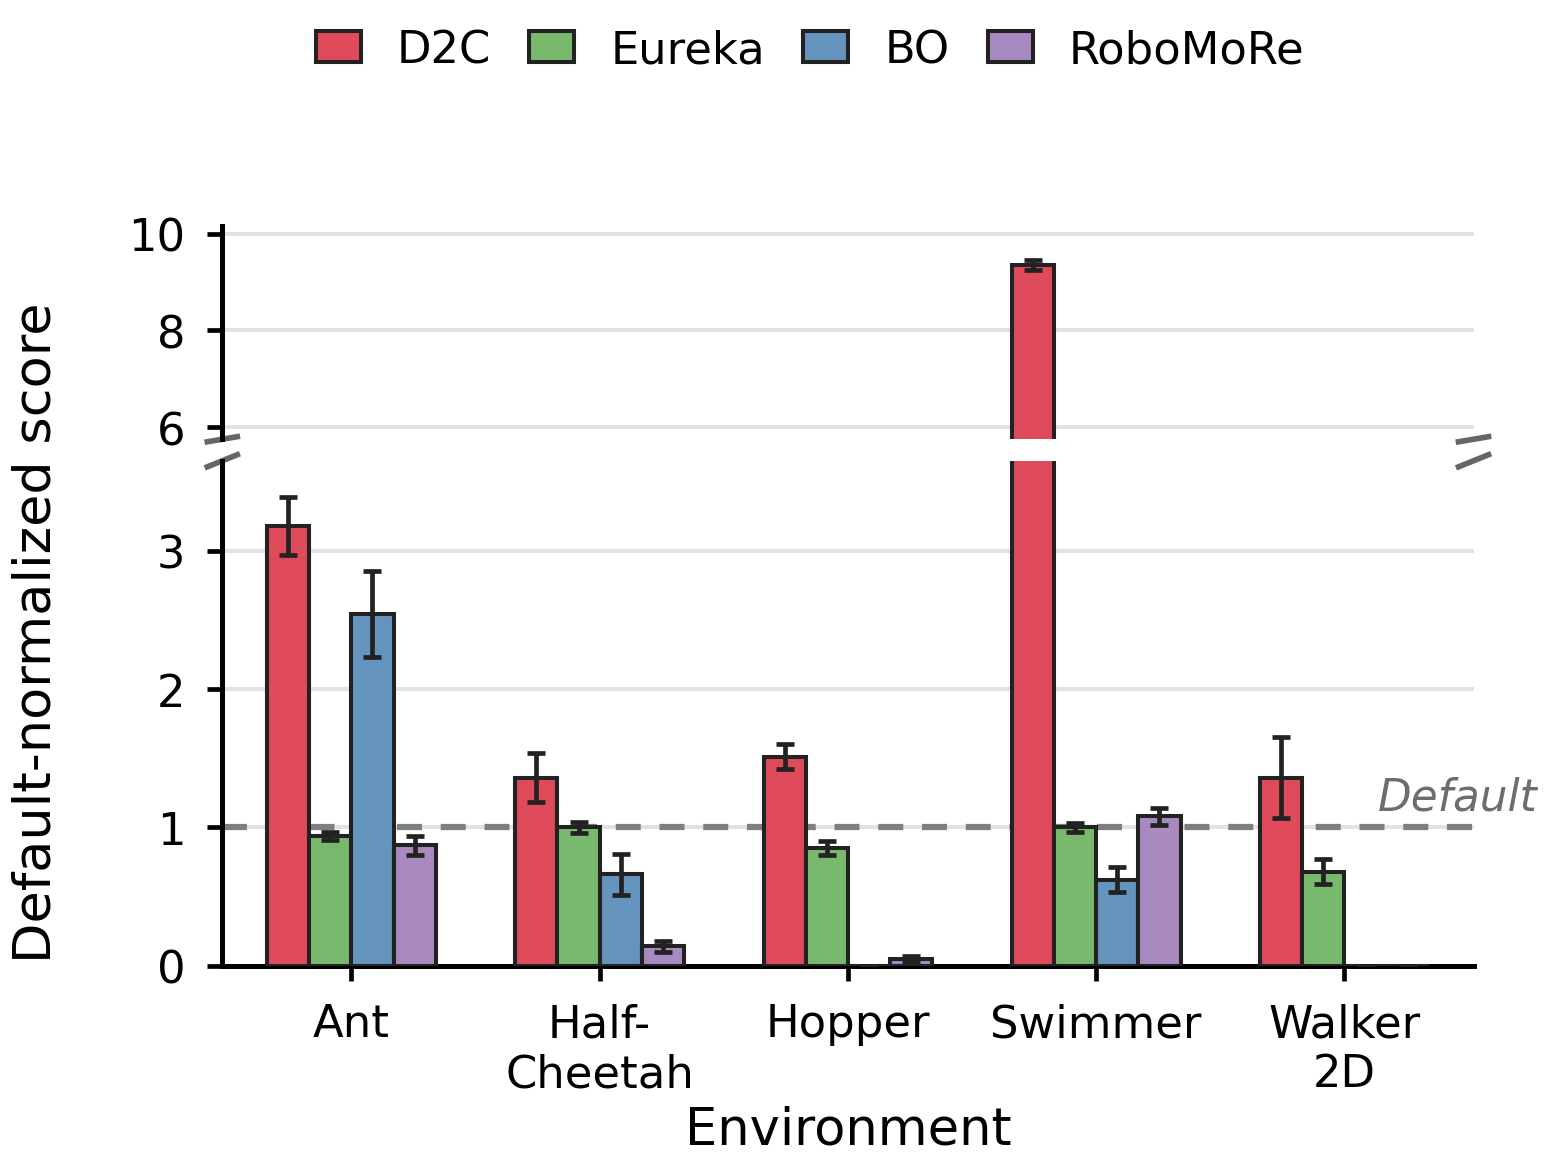
\includegraphics[width=\columnwidth]{figures/meta_normalized_bar.png}
    \caption{Default-normalized performance across environments (mean $\pm$ std over 3 search seeds). The y-axis uses a broken scale so the Swimmer gain remains visible without compressing the remaining tasks. \textbf{Takeaway:} \abbrev{} achieves the highest score across all five evaluated tasks.}
    \label{fig:meta_normalized_bar}
\end{figure}

\textbf{\abbrev{} learns transferable reward shaping.} Table~\ref{tab:design_reward_ablation} isolates morphology and reward contributions. Applying the \abbrev{} reward on the default morphology improves performance in 4/5 environments, suggesting the learned reward shaping is not tied to the discovered morphology. This transferability indicates that debate identifies reusable shaping patterns (e.g., stability maintenance, smooth actuation) rather than only morphology-specific rewards. The strongest results arise when both design and reward are produced by \abbrev{}, which outperforms the cross-over conditions in all tasks except Swimmer. In Swimmer, morphology changes alone yield ${\sim}10\times$ gains, leaving little room for reward shaping due to its low-DOF dynamics.

\textbf{Co-design interaction.} Table~\ref{tab:design_reward_ablation} exhibits non-additive interactions that suggest synergy between morphology and reward. We quantify this via a difference-in-differences term $\Delta_{\text{int}} = S(\text{\abbrev{}},\text{\abbrev{}}) - S(\text{\abbrev{}},\text{Def.}) - S(\text{Def.},\text{\abbrev{}}) + S(\text{Def.},\text{Def.})$. This term is positive in 4/5 tasks (e.g., Hopper: $\Delta_{\text{int}} = 1380$), indicating that \abbrev{}'s reward shaping is most effective when paired with the morphology it was co-designed for. Swimmer is the exception, consistent with its morphology-dominated gains.

\textbf{Per-environment analysis.} Ant shows large gains ($3.2\times$) due to a rich design space where wider stances and longer limbs improve stability at speed. Swimmer achieves the largest gains (${\sim}9\times$) because its low-DOF dynamics make morphology changes disproportionately impactful. HalfCheetah, Hopper, and Walker2D show modest gains ($1.3$--$1.5\times$) as bipedal dynamics impose tighter stability constraints. In these environments, reward shaping contributes a larger fraction of improvement (Table~\ref{tab:design_reward_ablation}).

\subsection{Debate Dynamics}
\label{sec:debate_dynamics}
\textbf{\abbrev{} improves over debate rounds.}
Figure~\ref{fig:best_scores_over_rounds} shows best-so-far improvement over rounds across all five environments, along with the Default-normalized baseline (1.0) and a zero-shot reference that generates 80 candidates without iterative feedback. Performance improves over rounds across all tasks, with \abbrev{} continuing to improve in later rounds (3--5). Appendix~\ref{app:debate-transcript} (Figure~\ref{fig:debate-morphology}) illustrates this progression for Ant: the best-performing morphology evolves from a compact design to one with a smaller torso, longer legs, and wider stance. To illustrate the debate dynamics: in Round 0, the stability judge noted ``marginal upright stability with increased contact,'' prompting the design agent to widen the stance ($0.22 \to 0.30$) and increase torso radius ($0.14 \to 0.16$), yielding a 33\% score improvement in Round 1.

\begin{figure*}[t]
    \centering
    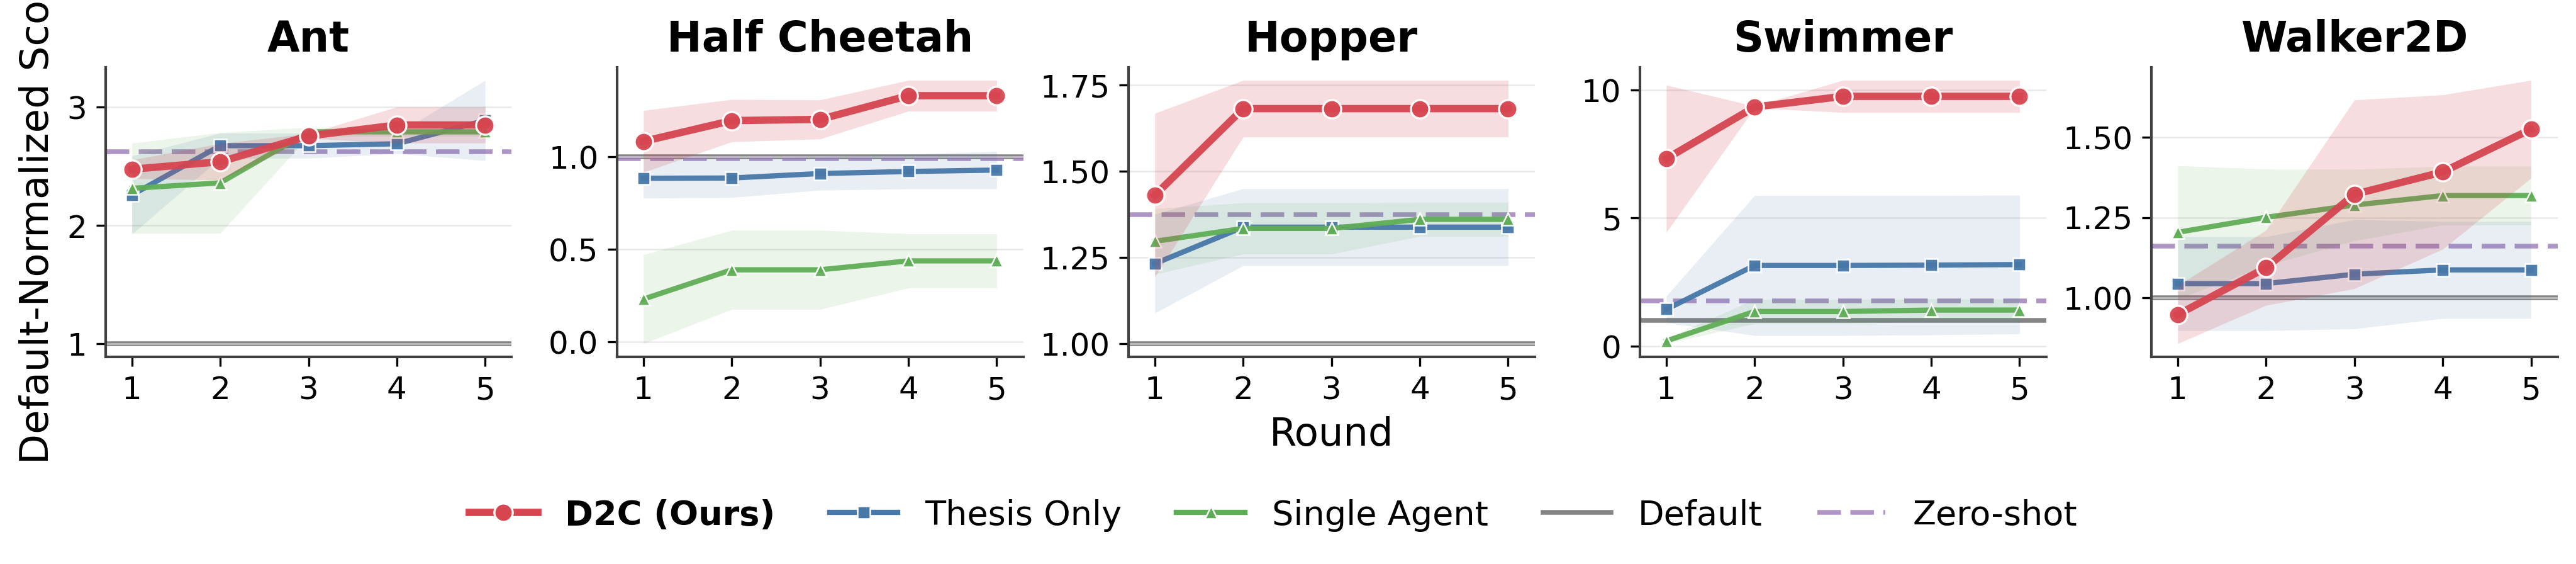
\includegraphics[width=0.95\textwidth]{figures/all_envs_best_scores_over_rounds_row.png}
\caption{Best-so-far Default-normalized scores over debate rounds (mean $\pm$ std over 3 search seeds). Dashed lines: Default baseline (1.0) and zero-shot (80 candidates, no iterative feedback). \textbf{Takeaway:} Iterative debate consistently improves over rounds, outperforming zero-shot generation by 18--35\%.}
    \label{fig:best_scores_over_rounds}
\end{figure*}

\textbf{\abbrev{} generates diverse designs.}
Figure~\ref{fig:xml_designs} shows representative final morphologies across tasks. \abbrev{} proposes non-trivial edits to limb lengths, torso proportions, and joint placements that reflect task-specific trade-offs (e.g., longer stride vs.\ stability). These are not simple scaling of the default model. The variety in final designs suggests that debate explores distinct regions of the design space rather than converging to a single canonical shape. In contrast, BO lacks semantic understanding of physical constraints, leading to ${\sim}12\%$ invalid morphology proposals compared to ${<}2\%$ for \abbrev{} (Appendix~\ref{app:baselines}).

\begin{figure*}[t]
    \centering
    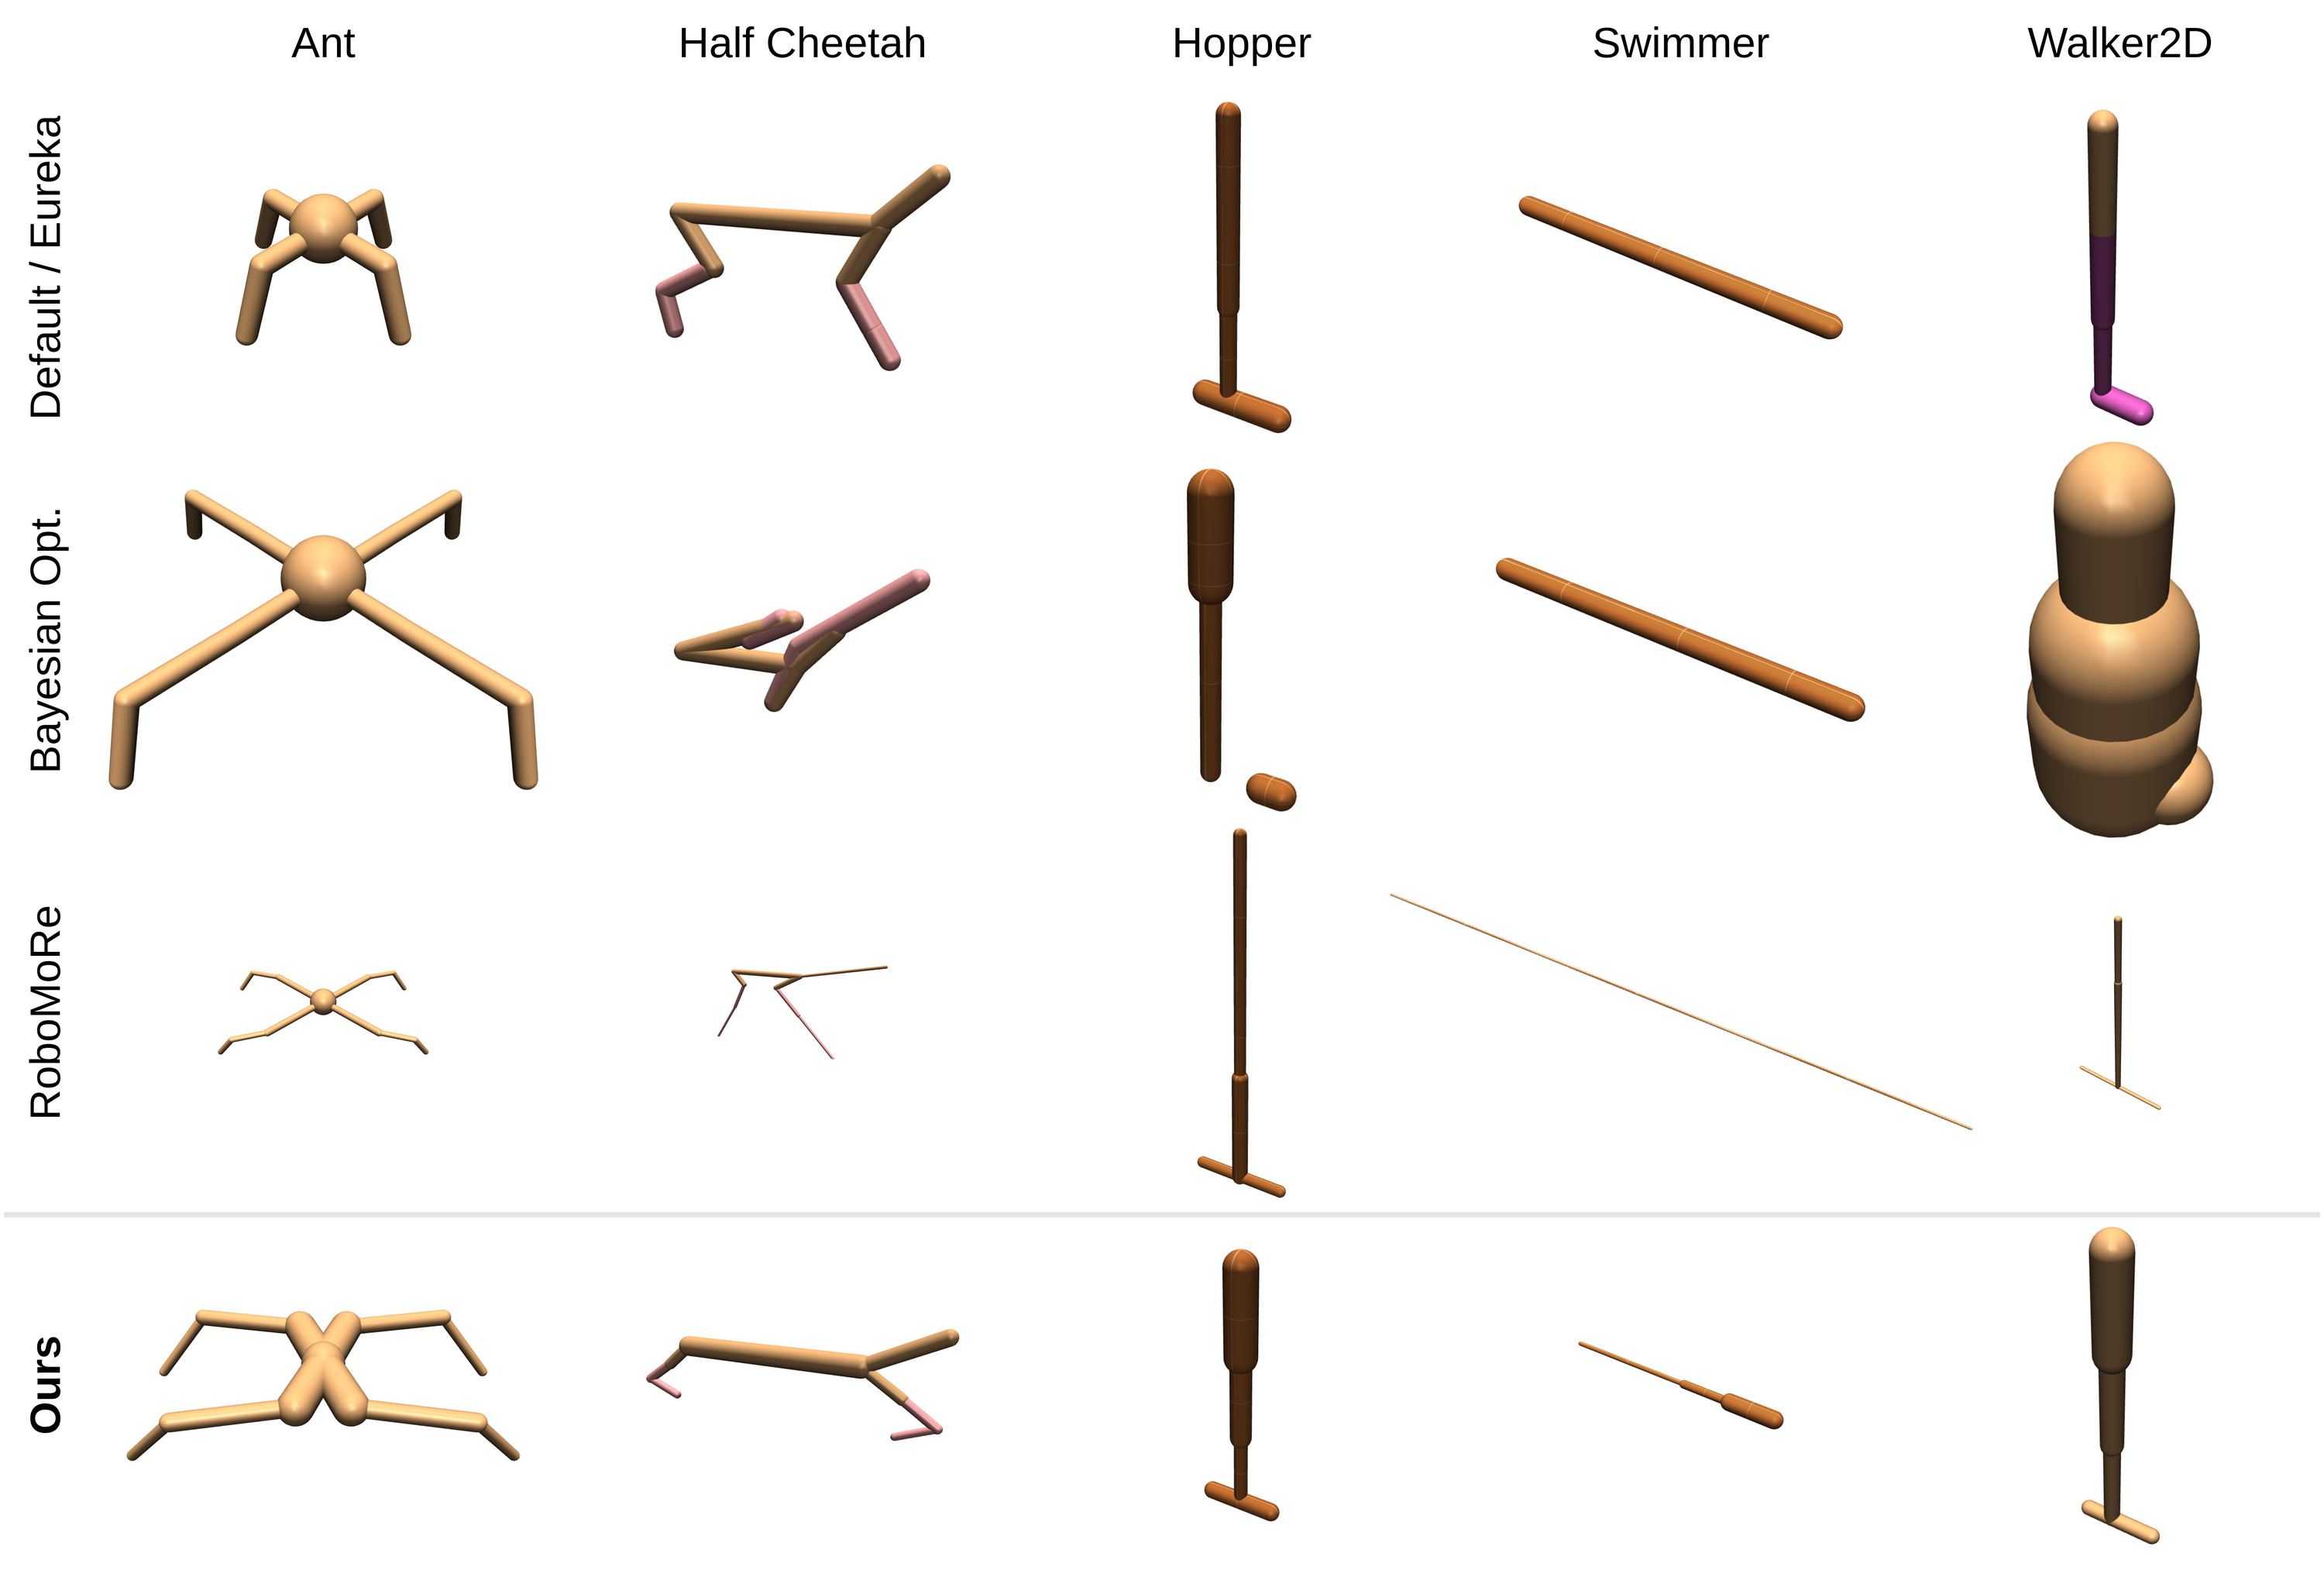
\includegraphics[width=0.9\textwidth]{figures/xmldesigns.png}
    \caption{Representative final morphologies across tasks. \abbrev{} discovers non-trivial modifications (longer legs and wider stance on Ant, extended torso on HalfCheetah, asymmetric limbs on Walker2D) while baselines produce more conservative or invalid designs.}
    \label{fig:xml_designs}
\end{figure*}

\textbf{\abbrev{} generates structurally distinct reward functions.}
Table~\ref{tab:design_reward_ablation} shows that the learned reward shaping improves performance even on the default morphology, indicating effects beyond morphology changes alone. To characterize structural differences, Figure~\ref{fig:reward_similarity} reports cosine similarity between reward-code feature vectors extracted via AST parsing. We extract term frequency vectors over reward components such as velocity bonuses, stability penalties, and energy costs (see Appendix~\ref{app:d2c_rewards} for details). Lower similarity for \abbrev{} indicates that its rewards use different combinations of shaping motifs than prior methods. Exact \abbrev{} reward expressions are provided in Appendix~\ref{app:d2c_rewards}.

\begin{figure}[t]
    \centering
    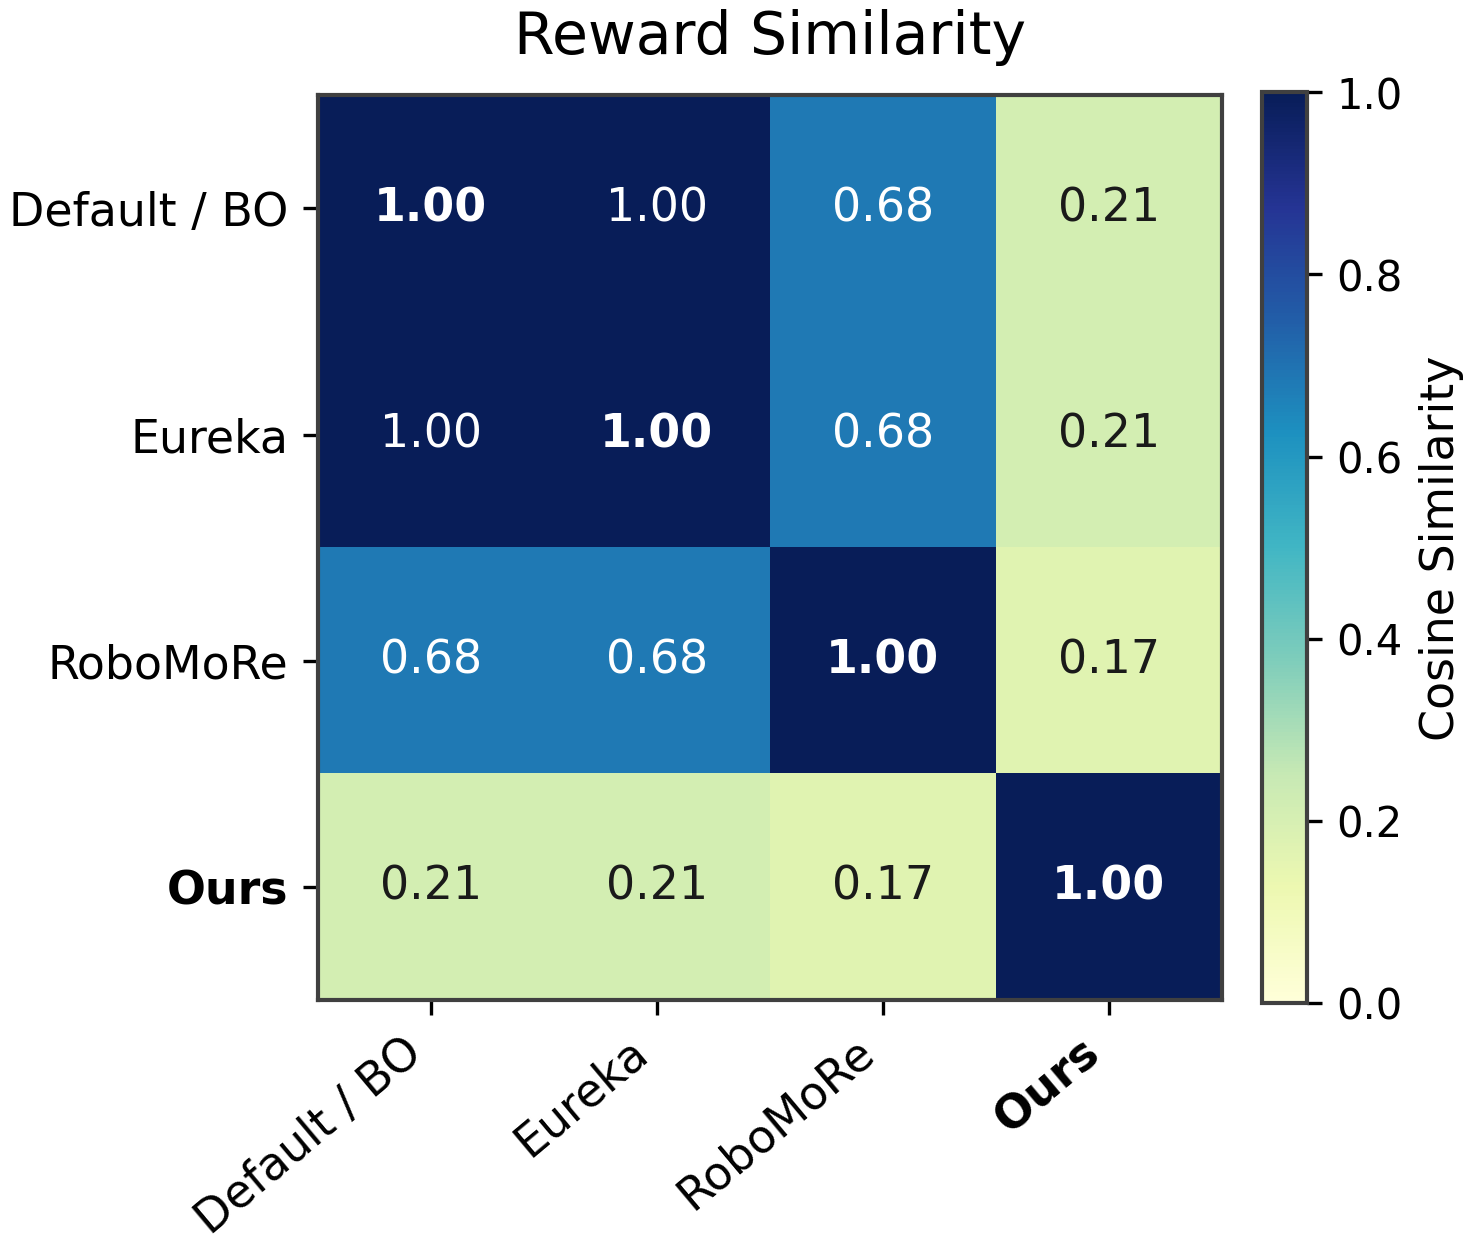
\includegraphics[width=0.81\columnwidth]{figures/reward_similarity_all.png}
    \caption{Reward-code similarity across methods (cosine similarity on AST-parsed feature vectors). Lower values indicate more distinct reward structures. Per-environment breakdown in Appendix~\ref{app:d2c_rewards}.}
    \label{fig:reward_similarity}
\end{figure}

\textbf{Common reward shaping patterns.} A post-hoc analysis of reward expressions (Appendix~\ref{app:d2c_rewards}) reveals recurring motifs. These include bounded nonlinearities to reduce reward hacking, smoothness penalties (4/5 environments) to stabilize novel morphologies, and orientation terms where debate identified balance as critical. Notably, backward-motion penalties emerged after the control agent observed oscillatory behaviors exploiting training reward. These patterns suggest debate can expose failure modes that single-pass generation misses. The consistency of these motifs across environments indicates that debate discovers reusable shaping strategies rather than only environment-specific heuristics.

\subsection{Ablation Studies}
\label{sec:ablation_studies}
We ablate three key components of \abbrev{}: iterative debate (vs.\ zero-shot), role separation (vs.\ single-agent), and criterion-specific judges (vs.\ no judges).

\textbf{Iterative debate outperforms zero-shot generation.} As shown in Figure~\ref{fig:best_scores_over_rounds}, the zero-shot baseline (dashed line) generates 80 candidates without iterative feedback. Despite identical candidate budgets, \abbrev{} surpasses the zero-shot optimum in later rounds (3--5), achieving 18--35\% higher scores (mean 24\%) across environments. This confirms that iterative critique and synthesis guide exploration beyond single-pass generation.

\textbf{Role separation and synthesis matter.} We evaluate two additional ablations (Figure~\ref{fig:best_scores_over_rounds}). In the \emph{single-agent} setting, one LLM proposes both morphology and reward without role specialization or cross-critique, but retains iterative rounds. In the \emph{thesis-only} setting, we disable synthesis and train only initial proposals. Both underperform full \abbrev{}: single-agent shows weaker improvement over rounds, while thesis-only plateaus early. These results support the role of specialization and critique-then-revise synthesis in sustaining gains beyond initial proposals.

\textbf{Judges influence design decisions.} We analyzed co-occurrence patterns between critique themes and parameter changes (Appendix~\ref{app:critique-analysis}). Chi-squared tests reveal significant associations ($p < 0.001$): speed critiques predict leg geometry changes, stability critiques predict leg and torso modifications. Runs with criterion-specific judges show smaller parameter change magnitudes than without judges ($0.126 \pm 0.102$ vs.\ $0.220 \pm 0.134$), suggesting more targeted refinements.

\textbf{Criterion-specific judges improve multi-objective coverage.}
Figure~\ref{fig:ablation_and_diversity_all} reports Pareto hypervolume~\cite{zitzler1998multiobjective, zitzler2003performance}. In environments with multi-dimensional trade-offs (Ant, Hopper, Walker2D), we compute 3D hypervolume over distance, stability, and efficiency, observing that criterion-specific judges improve coverage in all three. In HalfCheetah and Swimmer, the environments are inherently upright, so stability is less informative and hypervolume reduces to 2D. In these environments, the stability judge still provides feedback that does not influence outcomes, which may dilute useful critiques. A fairer comparison would remove the stability judge entirely for inherently stable tasks.

\textbf{LLM backbone sensitivity.} We evaluated three GPT-5 scales (nano, mini, full) on Ant to assess whether \abbrev{}'s gains depend on LLM capability. All models achieve comparable final archived scores ($3.18$--$3.60\times$ normalized; pairwise $t$-tests $p > 0.19$), suggesting that performance stems from the debate framework rather than raw model scale. However, smaller models produce substantially more degenerate candidates: GPT-5-mini has a $49.2\%$ failure rate (near-zero scores) versus $15.8\%$ for GPT-5.2. The archive mechanism makes \abbrev{} robust to individual failures, but smaller models waste computation on unviable designs.

\textbf{Open-weight backbones.} Appendix~\ref{app:open_weight_backbones} extends this analysis to two DeepSeek open-weight backbones on Ant and Swimmer under the same 3-seed, 80-candidate protocol. DeepSeek-R1 reaches $2.47\times$ and $6.62\times$ the Default baseline on Ant and Swimmer, while DeepSeek-V3 reaches $1.85\times$ and $3.72\times$, indicating that the debate loop remains useful without the proprietary main backbone, although absolute performance still trails GPT-5.2.

\begin{figure*}[t]
    \centering
    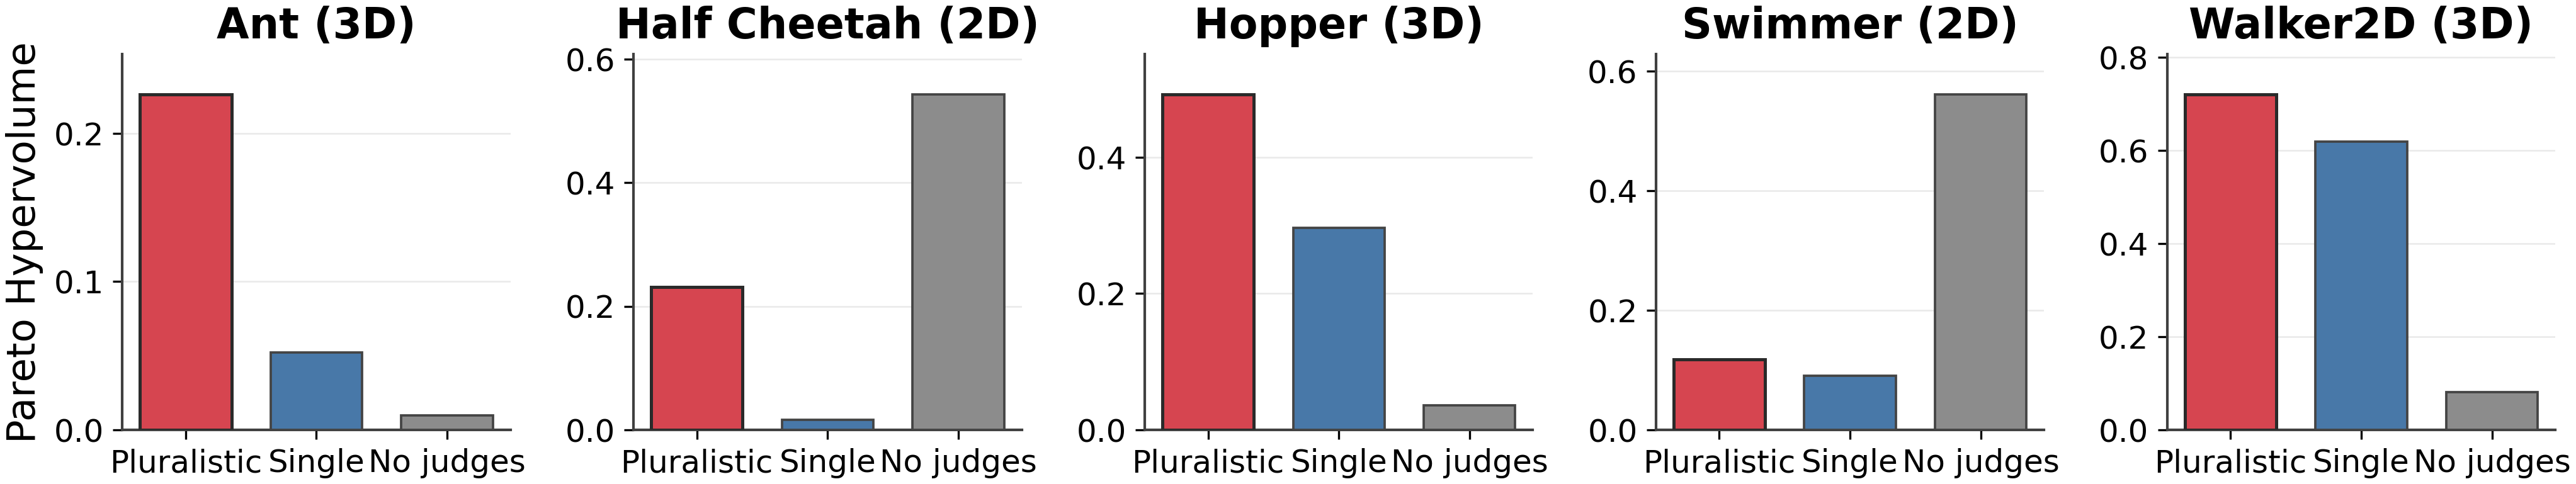
\includegraphics[width=0.96\textwidth]{figures/ablation_diversity_grid.png}
    \caption{Pareto hypervolume over multi-objective metrics (3 search seeds, higher = broader coverage). Environments where stability is meaningful (Ant, Hopper, Walker2D) use 3D hypervolume (distance, stability, efficiency); others (HalfCheetah, Swimmer) use 2D (distance, efficiency). \textbf{Takeaway:} Criterion-specific judges improve coverage in environments with meaningful multi-dimensional trade-offs.}
    \label{fig:ablation_and_diversity_all}
\end{figure*}
